\documentclass[12pt]{article}
\usepackage{extsizes}
\usepackage[brazil]{babel}
\usepackage{tikz}
\usepackage{graphicx}
\usepackage{caption}
\usepackage{subcaption}
\usepackage{stanli}
\usepackage{siunitx}
\usepackage{mathtools}
\usepackage{quotes}
\usepackage{amsmath}
\usepackage{empheq}
\usepackage{fancyhdr}
\usepackage{amsthm}
\usepackage{booktabs}
\usepackage{indentfirst}
\usepackage[a4paper,lmargin=1.75cm,rmargin=1.75cm,tmargin=2.5cm,bmargin=2.5cm]{geometry}

\begin{document}
\fancyhead[L]{PEF3208: Fundamentos em Mecânica das Estruturas}
\fancyhead[R]{Escola Politécnica - USP}
\fancyfoot[C]{\thepage}
\renewcommand{\headrulewidth}{0.4pt}
\renewcommand{\footrulewidth}{0pt}
\pagestyle{fancy}
\thispagestyle{plain}

\begin{center}
  {\LARGE\bfseries Sistema de suspensão rocker-bogie}\\

  \bigskip

  {\large Natanael Magalhães Cardoso}\\
  nUSP: 8914122

  \medbreak

  Relatório Final - Turma 03\\
  PEF3208: Fundamentos em Mecânica das Estruturas\\
  Prof. Osvaldo Shigueru Nakao\\
  \bigskip
  \today
\end{center}

\renewenvironment{abstract}
{\quotation\small\noindent\rule{\linewidth}{.5pt}\par\smallskip
  {\centering\bfseries\abstractname\par}\medskip}
{\par\noindent\rule{\linewidth}{.5pt}\endquotation}

\begin{abstract}
  Este projeto consiste na aplicação dos conceitos da disciplina PEF3208 para analisar uma estrutura real. A estrutura escolhida foi o sistema de suspensão rocker-bogie, projetado e usado pela NASA em diversas missões de exploração de Marte.
\end{abstract}

\section{Introdução}

\newlength{\currentparskip}
\newlength{\currentparindent}
\setlength{\currentparskip}{\parskip}
\setlength{\currentparindent}{\parindent}
\begin{minipage}{.53\textwidth}
  \setlength{\parskip}{\currentparskip}
  \setlength{\parindent}{\currentparindent}
  O sistema de suspensão rocker-bogie foi projetado em 1988 por Donald B. Bickler para o uso da NASA no veículo espacial Sojourner. E, desde então, tornou-se o sistema de suspensão preferido da companhia para explorações espaciais, tendo sido reutilizado em outras missões como Mars 2003, Mars 2012 e Mars 2020 (figura \ref{fig:int-1}).
  \medskip

  A parte \emph{rocker} (oscilante) da suspensão vem do aspecto oscilante da articulação maior montada no corpo em cada lado do veículo espacial. Esses balancins são conectados um ao outro e ao chassi do veículo através de um diferencial. Em relação ao chassi, os balancins girarão em direções opostas para manter um contato aproximadamente igual com a roda. O chassi mantém o ângulo de inclinação médio dos dois balancins. Uma extremidade de um balancim é equipada com uma roda motriz e a outra extremidade é articulada ao bogie.
  \medskip

  A parte \emph{bogie} da suspensão refere-se à ligação menor, que gira para o balancim no meio e que tem uma roda motriz em cada extremidade. Os bogies eram comumente usados como rodas de carga nos trilhos dos tanques do exército como roldanas que distribuíam a carga no terreno e também eram comumente usados em reboques de caminhões semi-reboques. Agora, tanques e semi-reboques preferem suspensões de braço à direita.
\end{minipage}%
\hfill%
\begin{minipage}{.4\textwidth}
  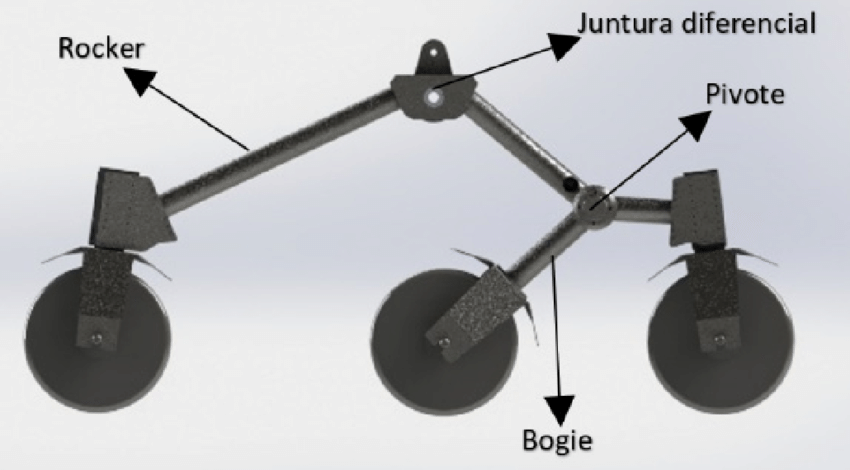
\includegraphics[width=\linewidth,height=3.4cm]{fig/rb-suspension.png}
  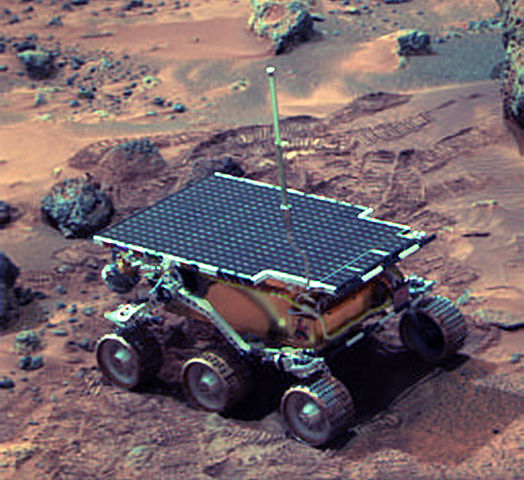
\includegraphics[width=.49\linewidth,height=3cm]{fig/sojourner.jpg}
  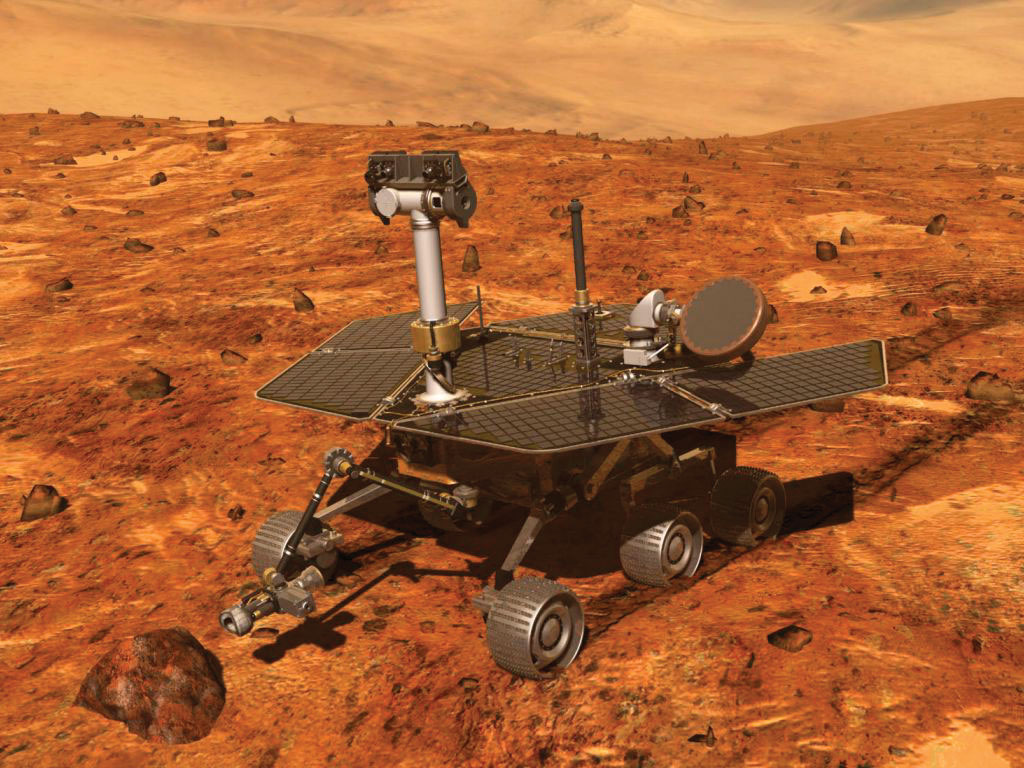
\includegraphics[width=.49\linewidth,height=3cm,trim={6cm 0 0 0},clip]{fig/spirit.jpg}
  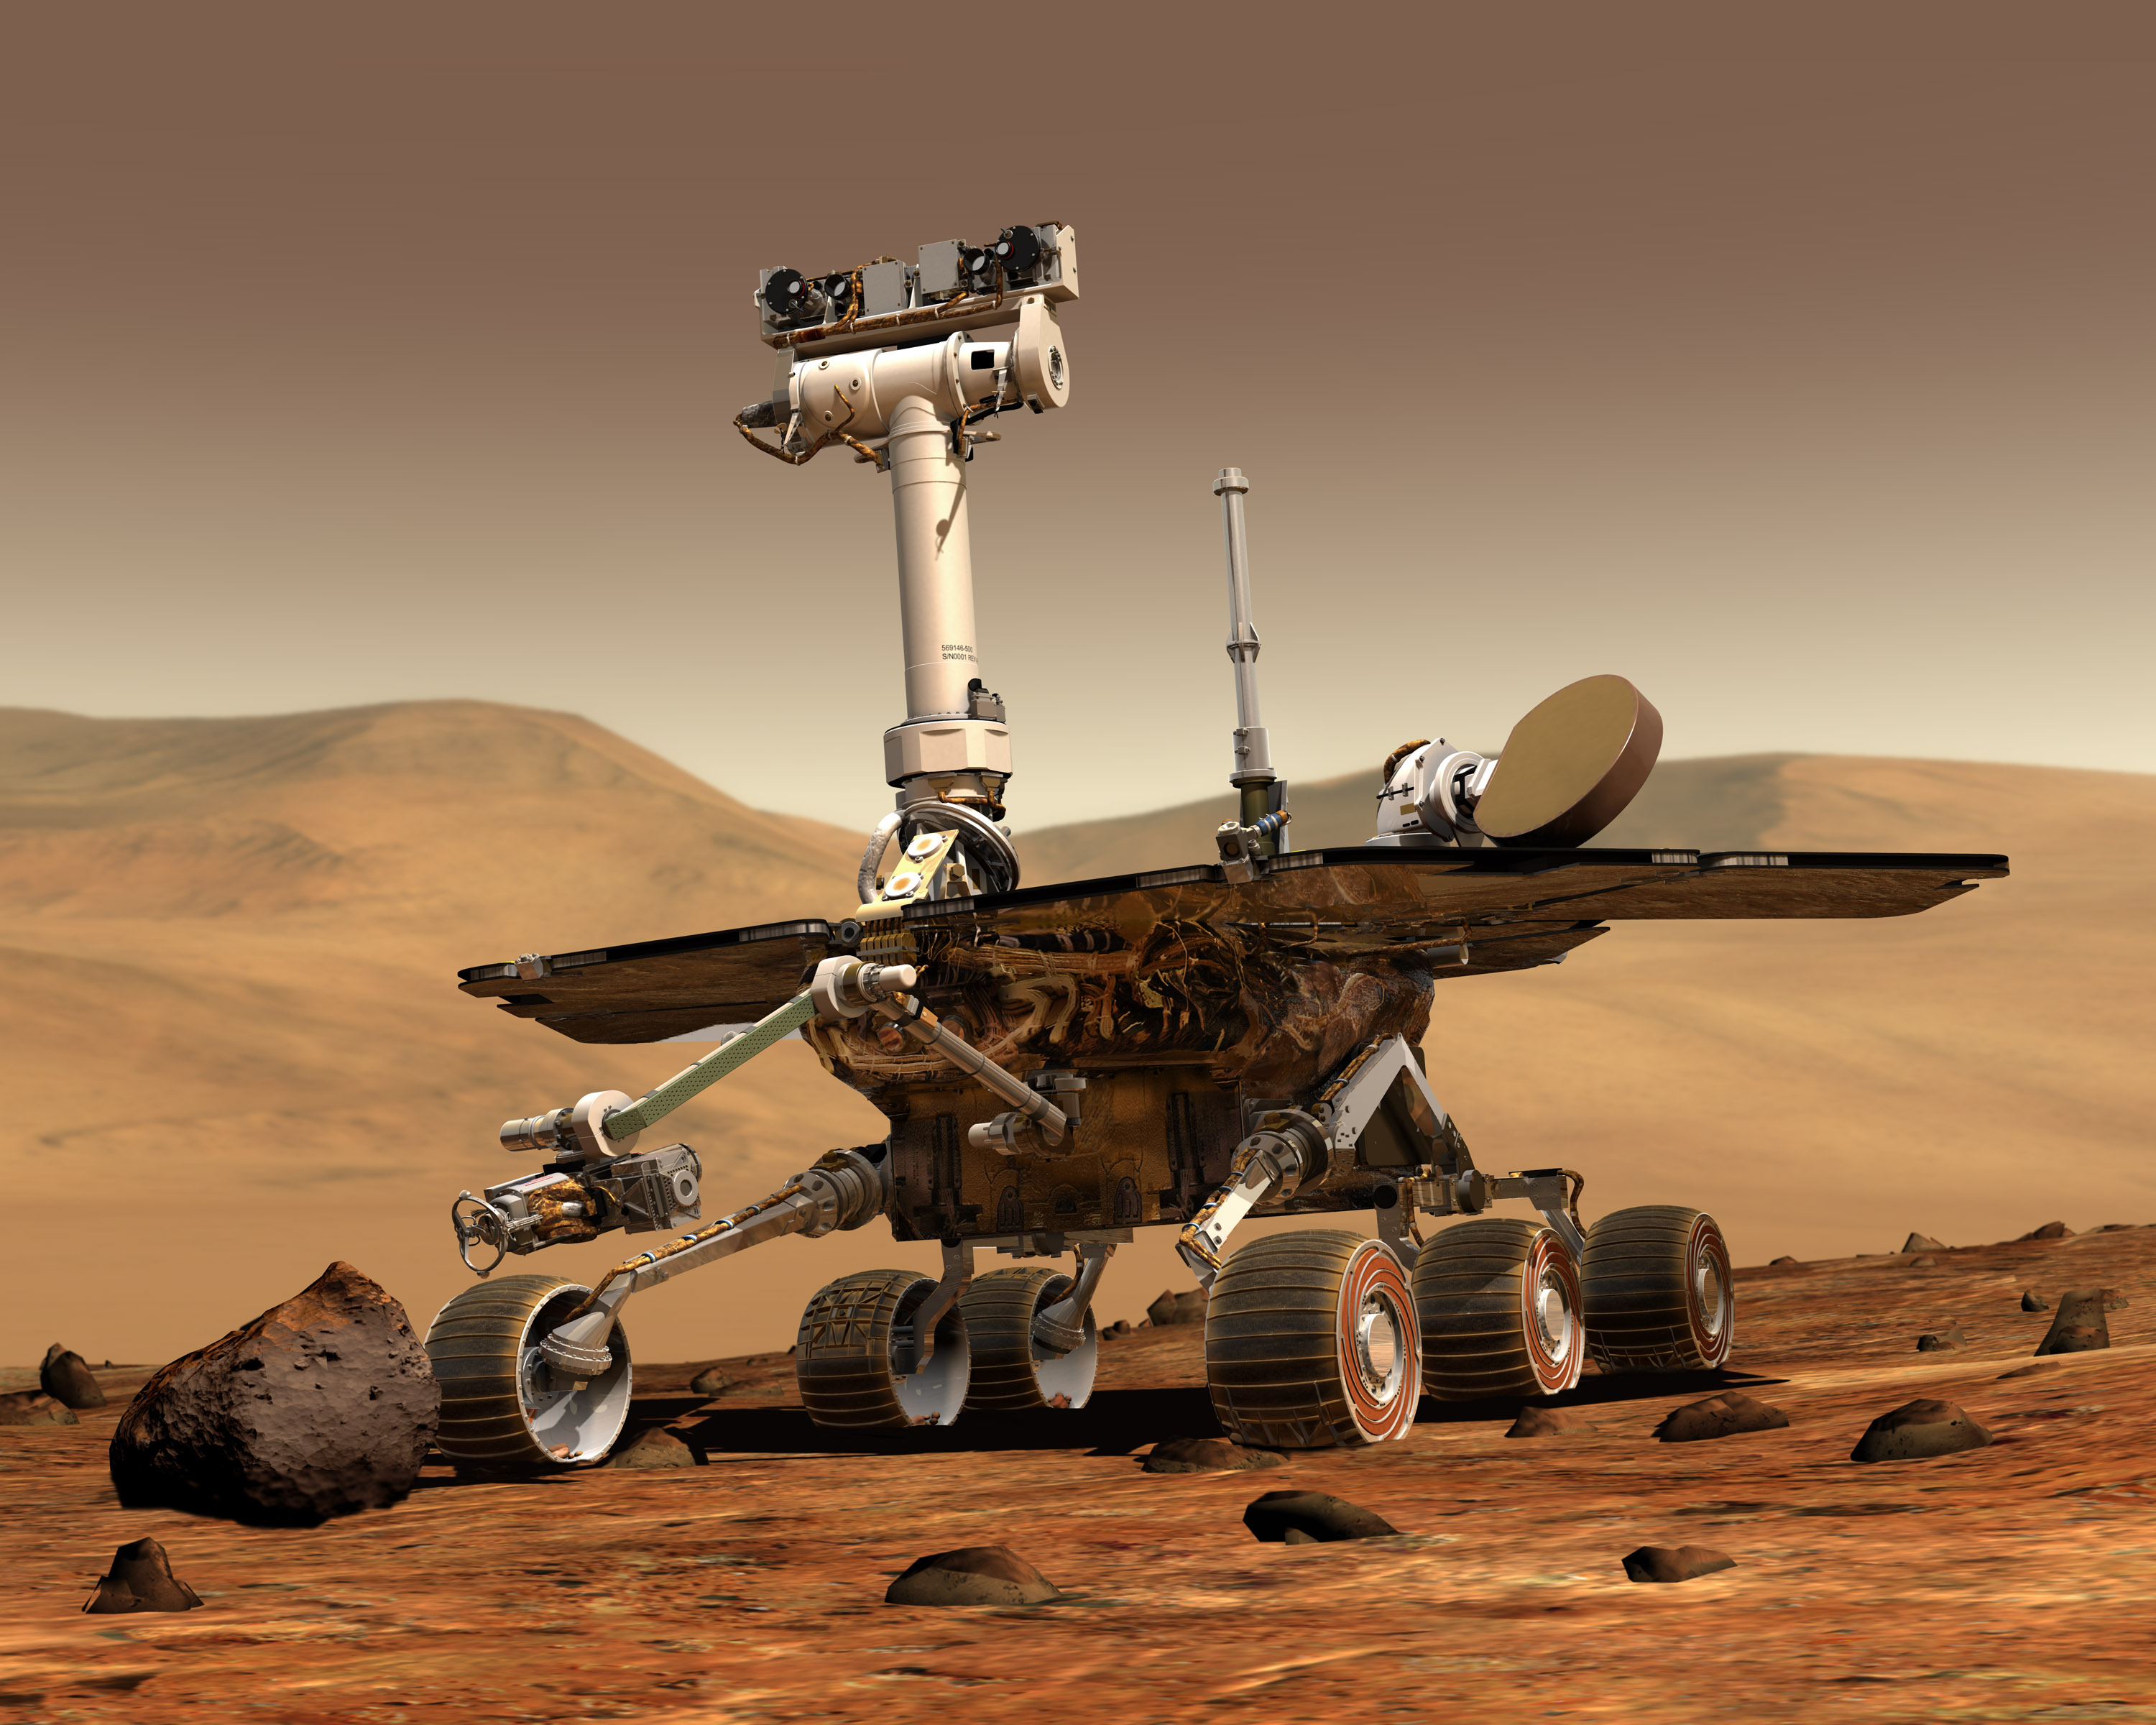
\includegraphics[width=.49\linewidth,height=3cm]{fig/opportunity.jpg}
  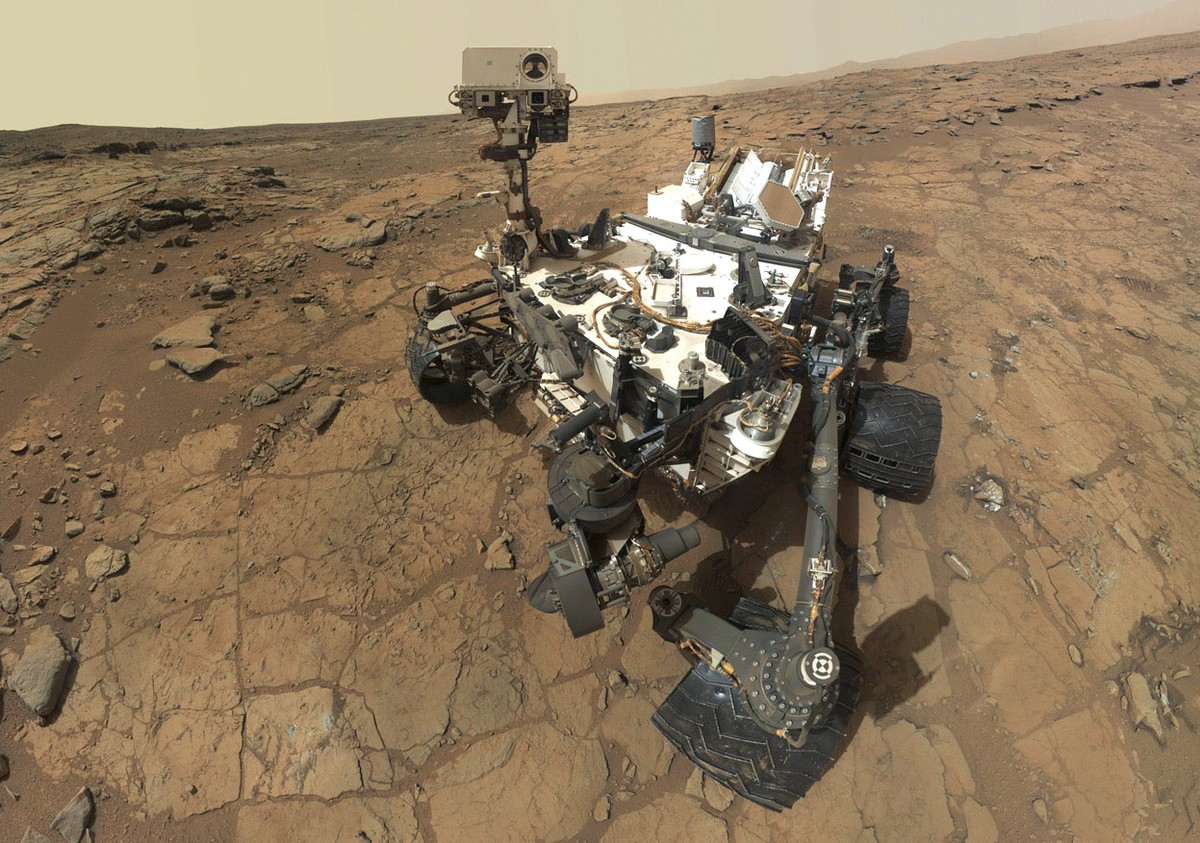
\includegraphics[width=.49\linewidth,height=3cm,trim={12cm 0 7cm 0},clip]{fig/curiosity.jpg}
  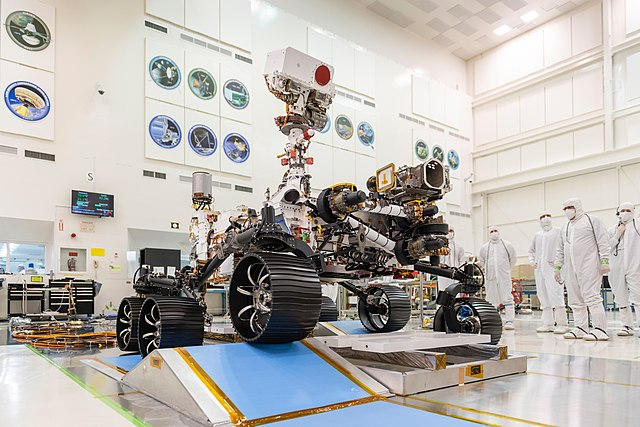
\includegraphics[width=\linewidth,height=3.5cm,trim={0 2.7cm 0 1.5cm},clip]{fig/perseverance.jpg}
  \captionof{figure}{Sistema rocker-bogie, Sojourner (1996), Spirit (2003), Opportunity (2003), Curiosity (2011) e Perseverance (2020).}
  \label{fig:int-1}
\end{minipage}

\pagebreak

\section{Definição da Estrutura}

Uma possível representação do sistema rocker-bogie é pela estrutura da figura \ref{fig:diagrama-base}. Comparando-a com a figura \ref{fig:int-1}, podemos identificar alguns componentes: o ponto E representa a junta diferencial é ele que recebe a carga do veículo; o ponto de refere-se ao pivot; o segmento AE representa a rocker e o segmento BD representa o bogie.

\begin{figure}[h!]
  \centering
  \resizebox{.6\textwidth}{!}{\begin{tikzpicture}
  \begin{scope}
    \point{a}{0}{0};
    \point{b}{5}{0};
    \point{c}{10}{0};
    \point{d}{7.5}{2.5};
    \point{e}{5}{5};

    \beam{2}{a}{e};
    \beam{2}{e}{c};
    \beam{2}{d}{b};

    \support{2}{a};
    \support{2}{b};
    \support{1}{c};

    \dimensioning{1}{a}{b}{-2}[L/2];
    \dimensioning{1}{b}{d}{-2}[L/4];
    \dimensioning{1}{d}{c}{-2}[L/4];
    \dimensioning{2}{d}{e}{11.5}[h/2];
    \dimensioning{2}{c}{d}{11.5}[h/2];

    \load{1}{e}[90];

    \dnotation{1}{e}{P}[yshift=9mm,right=1mm];
    \dnotation{1}{a}{A}[above left];
    \dnotation{1}{b}{B}[above left];
    \dnotation{1}{c}{C}[above right];
    \dnotation{1}{d}{D}[above right];
    \dnotation{1}{e}{E}[below=2mm];
  \end{scope}
\end{tikzpicture}}
  \smallskip
  \caption{Estrutura representando uma suspensão rocker-bogie.}
  \label{fig:diagrama-base}
\end{figure}

Mas, para resolver a estrutura, a simplificação da figura \ref{fig:diagrama-simpl} foi adotada. Ela consiste na separação da estrutura em duas mais simples. Para tanto, foi considerado que no ponto D da figura ADE existe um apoio fixo e as reações deste apoio são transferidas como carga para o ponto D da estrutura BCD.

\begin{figure}[h!]
  \centering
  \resizebox{.7\textwidth}{!}{\begin{tikzpicture}
  \begin{scope}
    \point{a}{0}{0};
    \point{b}{6.5}{-1.5};
    \point{c}{11.5}{-1.5};
    \point{d1}{7.5}{2.5};
    \point{d2}{9}{1};
    \point{e}{5}{5};

    \beam{2}{a}{e};
    \beam{2}{d1}{e};
    \beam{2}{b}{d2};
    \beam{2}{c}{d2};

    \support{2}{a};
    \support{2}{b};
    \support{1}{c};
    \support{1}{d1};

    \dimensioning{1}{a}{e}{-4}[L/2];
    \dimensioning{1}{b}{d2}{-4}[L/4];
    \dimensioning{1}{d2}{c}{-4}[L/4];
    \dimensioning{2}{d1}{e}{13}[h/2];
    \dimensioning{2}{c}{d2}{13}[h/2];

    \load{1}{e}[90];

    \dnotation{1}{e}{P}[yshift=9mm,right=1mm];
    \dnotation{1}{a}{A}[above left];
    \dnotation{1}{b}{B}[above left];
    \dnotation{1}{c}{C}[above right];
    \dnotation{1}{d1}{D}[above right];
    \dnotation{1}{d2}{D}[below=2mm];
    \dnotation{1}{e}{E}[below=2mm];

    \draw[-{latex[scale=3.0]},very thick] (7.5,0.75) -- (7.5,1.65) node[yshift=-3mm,left=8mm] {H\textsubscript{D}};
    \draw[-{latex[scale=3.0]},very thick] (6.3,1.55) -- (7.3,1.55) node[yshift=-8mm,left=-3mm] {V\textsubscript{D}};
    \load{1}{d2}[90];
    \dnotation{1}{d2}{H\textsubscript{D}}[yshift=2mm,right=8mm];
    \load{1}{d2}[360];
    \dnotation{1}{d2}{V\textsubscript{D}}[yshift=11mm,right=-1mm];
  \end{scope}
\end{tikzpicture}}
  \smallskip
  \caption{Redução da estrutrua da figura \ref{fig:diagrama-base} em duas estrutras mais simples.}
  \label{fig:diagrama-simpl}
\end{figure}

\pagebreak

\section{Resolução da Estrutura}

\begin{minipage}{.48\textwidth}
  Para analisar os esforços internos do sistema de suspensão rocker-bogie, primeiro iremos calcular as reações nos apoios de cada estrutura, para, então, gerar as equações dos esforços solicitantes a partir do Teorema do Corte. Para todos os cálculos desta seção, será considerada a convenção da figura \ref{fig:convencoes}(a) para esforços solicitantes e a convenção de Grinter para o equilíbrio, figura \ref{fig:convencoes}(b).
  \end{minipage}%
\hfill%
\begin{minipage}{.45\textwidth}
  \begin{minipage}{.7\textwidth}
    \centering
    \resizebox{\linewidth}{!}{\begin{tikzpicture}
  \draw[fill=blue!60,color=blue!60] (0,0) rectangle (.6,1);
  \draw[->] (.7,.8) -- (1.4,.8) node[above] {\tiny $N$};
  \draw[->] (.7,.8) -- (.7,.1) node[below] {\tiny $V$};
  \path[->] (.8,.1) edge[bend right=45] (1.4,.7) node[below right,yshift=1mm] {\tiny $M$};
  \draw (1,.5) node{+};

  \draw[->] (2.3,.2) -- (1.6,.2) node[below] {\tiny $N$};
  \draw[->] (2.3,.2) -- (2.3,.9) node[above] {\tiny $V$};
  \path[->] (1.6,.3) edge[bend left=45] (2.2,.9);
  \draw[fill=blue!60,color=blue!60] (2.4,0) rectangle (3,1);
  \draw (2,.5) node{+};
\end{tikzpicture}}
    (a)
  \end{minipage}%
  \hfill%
  \begin{minipage}{.25\textwidth}
    \centering
    \resizebox{\linewidth}{!}{\begin{tikzpicture}
  \draw[->] (-.1,0) -- (1,0);
  \draw[->] (0,-.1) -- (0,1);
  \path[->] (1,.2) edge[bend right=25] (.2,1);
  \draw (.4,.4) node[anchor=center] {\large +};
\end{tikzpicture}}
    (b)
  \end{minipage}
  \captionof{figure}{Convenções adotadas.}
  \label{fig:convencoes}
\end{minipage}


\subsection{Reações nos apoios em ADE}

\begin{figure}[h!]
  \centering
  \resizebox{.5\linewidth}{!}{\begin{tikzpicture}
  \begin{scope}
    \point{a}{0}{0};
    \point{b}{6.5}{-1.5};
    \point{c}{11.5}{-1.5};
    \point{d1}{7.5}{2.5};
    \point{d2}{9}{1};
    \point{e}{5}{5};

    \beam{2}{a}{e};
    \beam{2}{d1}{e};

    \support{2}{a};
    \support{1}{d1};

    \dimensioning{1}{a}{e}{-2.5}[L/2];
    \dimensioning{1}{e}{d1}{-2.5}[L/4];
    \dimensioning{2}{a}{d1}{9}[h/2];
    \dimensioning{2}{d1}{e}{9}[h/2];

    \load{1}{e}[90];

    \dnotation{1}{e}{P}[yshift=9mm,right=1mm];
    \dnotation{1}{a}{A}[above left];
    \dnotation{1}{d1}{D}[above right];
    \dnotation{1}{e}{E}[below=2mm];

    \draw[-{latex[scale=3.0]},very thick] (7.5,0.75) -- (7.5,1.65) node[yshift=-3mm,left=8mm] {$H_D$};
    \draw[-{latex[scale=3.0]},very thick] (6.3,1.55) -- (7.3,1.55) node[yshift=-8mm,left=-3mm] {$V_D$};
    \load{1}{a}[270][.9][1];
    \dnotation{1}{a}{$V_A$}[left=-1mm,yshift=-18mm];

    \draw[-{latex[scale=3.0]},thick] (.8,0) arc (0:45:.8) node[] at (20:1.1) {$\alpha$};
    \draw[dashed] (0,0) -- (2,0);
    \draw[-{latex[scale=3.0]},thick] (6.7,2.5) arc (180:135:.8) node[shift=({7.5,2.5})] at (160:1.1) {$\beta$};
    \draw[dashed] (7.5,2.5) -- (5.5,2.5);
  \end{scope}
\end{tikzpicture}}
  \caption{Estrutura AED.}
  \label{fig:aed}
\end{figure}

\begin{empheq}[left=\empheqlbrace]{align*}
  &\sum F_H = 0 \;\Rightarrow\; H_D = 0\\
  &\sum F_V = 0 \;\Rightarrow\; V_A + V_D - P = 0\\
  &\sum M_A = 0 \;\Rightarrow\; \left(\frac{L}{2} + \frac{L}{4}\right)V_D - \frac{L}{2}P - \frac{h}{2}H_D = 0\\
  &\sum M_D = 0 \;\Rightarrow\; \left(\frac{L}{2} + \frac{L}{4}\right)V_A + \frac{L}{4}P = 0
\end{empheq}
\begin{center}
  $\boxed{H_D = 0}$ \qquad $\boxed{V_A = \frac{P}{3}}$ \qquad $\boxed{V_D = \frac{2P}{3}}$
\end{center}

\pagebreak

\subsection{Reações nos apoios em BCD}

\begin{figure}[h!]
  \centering
  \resizebox{.5\textwidth}{!}{\begin{tikzpicture}
  \begin{scope}
    \point{a}{0}{0};
    \point{b}{6.5}{-1.5};
    \point{c}{11.5}{-1.5};
    \point{d1}{7.5}{2.5};
    \point{d2}{9}{1};
    \point{e}{5}{5};

    \beam{2}{b}{d2};
    \beam{2}{c}{d2};

    \support{2}{b};
    \support{1}{c};

    \dimensioning{1}{b}{d2}{-4}[L/4];
    \dimensioning{1}{d2}{c}{-4}[L/4];
    \dimensioning{2}{c}{d2}{13}[h/2];

    \dnotation{1}{b}{B}[above left];
    \dnotation{1}{c}{C}[above right];
    \dnotation{1}{d2}{D}[below=2mm];

    \load{1}{d2}[90];
    \dnotation{1}{d2}{H\textsubscript{D}}[yshift=2mm,right=8mm];
    \load{1}{d2}[360];
    \dnotation{1}{d2}{V\textsubscript{D}}[yshift=11mm,right=-1mm];
    \load{1}{b}[270][.9][1];
    \dnotation{1}{b}{V\textsubscript{A}}[left=-1mm,yshift=-19mm];
    \load{1}{c}[270][.9][1];
    \dnotation{1}{c}{V\textsubscript{C}}[right,yshift=-19mm];
    \draw[-{latex[scale=3.0]},very thick] (10.4,-2.5) -- (11.4,-2.5) node[below,xshift=-9mm] {H\textsubscript{C}};

    \draw[-{latex[scale=3.0]},thick] (7.3,-1.5) arc (0:45:.8) node[shift=({6.5,-1.5})] at (20:1.1) {$\gamma$};
    \draw[dashed] (6.5,-1.5) -- (7.9,-1.5);
    \draw[-{latex[scale=3.0]},thick] (10.7,-1.5) arc (180:135:.8) node[shift=({11.5,-1.5})] at (160:1.1) {$\delta$};
    \draw[dashed] (11.5,-1.5) -- (10.1,-1.5);
  \end{scope}
\end{tikzpicture}}
  \captionof{figure}{Estrutura BCD.}
  \label{fig:bcd}
\end{figure}

\begin{minipage}{.6\textwidth}
  \begin{empheq}[left=\empheqlbrace]{align*}
    &\sum F_H = 0 \;\Rightarrow\; -H_D + H_C = 0\\
    &\sum F_V = 0 \;\Rightarrow\; V_B + V_C - V_D = 0\\
    &\sum M_B = 0 \;\Rightarrow\; \frac{L}{2}V_C - \frac{L}{4}V_D = 0\\
    &\sum M_C = 0 \;\Rightarrow\; -\frac{L}{2}V_B + \frac{L}{4}V_D = 0
  \end{empheq}
\end{minipage}%
\hfill%
\begin{minipage}{.4\textwidth}
  \centering
  $\boxed{V_B = \frac{P}{3}}$ \qquad $\boxed{V_C = \frac{P}{3}}$\\
  $$\boxed{H_C = 0}$$
\end{minipage}

\bigskip
\bigskip

Os valores das reações nos apoios de ambas as estruturas serão dispostos na tabela seguinte para organizar a consulta na próxima etapa da análise.

\begin{table}[h!]
  \centering
  \begin{tabular}{cccc}
    \toprule
    \multicolumn{2}{c}{ADE} & \multicolumn{2}{c}{BCD}                                     \\
    Variável                & Valor (N)               & Variável    & Valor (N)           \\
    \midrule
    \large$H_D$             & \large 0                & \large$H_C$ & \large 0            \\[4pt]
    \large$V_A$             & \Large$\frac{P}{3}$     & \large$V_B$ & \Large$\frac{P}{3}$ \\[8pt]
    \large$V_D$             & \Large$\frac{2P}{3}$    & \large$V_C$ & \Large$\frac{P}{3}$ \\[8pt]
    \bottomrule
  \end{tabular}
  \caption{Valores das reações externas calculadas pelas equações de equilíbrio.}
  \label{tab:variaveis}
\end{table}

E, para prosseguir com a resolução da estrutura, os esforços internos serão calculados a seguir usando o Teorema do Corte.

\pagebreak

O sistema formado por essas seis equações não gera o número de equações LI suficientes para 
determinar os valores das 6 incógnitas, por isso acredito que as equações que escrevi estão erradas.
Gostaria de saber o que estou fazendo errado ou se existe uma forma melhor de fazer isso. 
Não sei se é melhor aplicar o método do equilíbrio dos nós.

\begin{empheq}[left=\empheqlbrace]{align}
  &\sum F_H = 0 \;\;\Rightarrow\;\; H_A + H_B + H_C = 0\\
  &\sum F_V = 0 \;\;\Rightarrow\;\; V_A + V_B + V_C - P = 0\\
  &\sum M^{(A)} = 0 \;\;\Rightarrow\;\; \frac{L}{2}V_A + LV_C - \frac{L}{2}P = 0\\
  &\sum M^{(B)} = 0 \;\;\Rightarrow\;\; -\frac{L}{2}V_A + \frac{L}{2}V_C = 0\\
  &\sum M^{(C)} = 0 \;\;\Rightarrow\;\; -LV_A - \frac{L}{2}V_B + \frac{L}{2}P = 0
\end{empheq}

\end{document}